\title{Sample Midterm Exam 2\ifsol\\[4pt]\large Answer Key\fi}
\author{Econ 5030}
\date{}

\begin{document}
\maketitle
\thispagestyle{myheadings}

\section{Preferences}

\noindent Consider an agent with preferences over $X=[0,1]\times[0,1]$ defined as follows: For all $x,x'\in X$,
\begin{align*}
x &\succ x' \text{ if } x_1 > x_1',\\
x &\succ x' \text{ if } x_1 = x_1' \text{ and } x_2 > x_2',\\
x &\sim x' \text{ if } x = x'.
\end{align*}

\begin{description}
\item[1.1] Write the definition of complete preferences and clearly demonstrate that these preferences are (or are not) complete on $X$.
\begin{solution}
Complete: for all $x,y\in X$, $x\succsim y$ or $y\succsim x$.

These (lexicographic) preferences \textbf{are complete}. Take any $x,y$. If $x_1\neq y_1$, the bundle with the larger first coordinate is strictly preferred. If $x_1=y_1$ and $x_2\ne y_2$, the bundle with the larger second coordinate is strictly preferred. If $x=y$, then $x\sim y$. Every pair is ranked.
\end{solution}
\item[1.2] Write the definition of transitive preferences and clearly demonstrate that these preferences are (or are not) transitive on $X$.
\begin{solution}
Transitive: $x\succsim y$ and $y\succsim z$ imply $x\succsim z$.

\textbf{Transitive.} $x\succsim y$ means $(x_1,x_2)$ is weakly above $(y_1,y_2)$ in dictionary order: first compare $x_1$, and use $x_2$ only to break ties. Suppose $x\succsim y\succsim z$. Then $x_1\ge y_1\ge z_1$. If $x_1>z_1$, then $x\succ z$. If $x_1=z_1$, then $x_1=y_1=z_1$, so $x_2\ge y_2\ge z_2$ and $x\succsim z$.
\end{solution}
\item[1.3] Does a utility function exist that represents these preferences on $X$? Explain.
\begin{solution}
\textbf{No.} The preferences are complete and transitive, but they are \emph{not continuous}. Take $x^n=(1/n,0)$ and $y^n=(0,1)$. Then $x^n\succ y^n$ for every $n$, but the limits satisfy $(0,0)\prec(0,1)$, so the preference ``jumps'' at the limit.

The intuition behind non-existence: each value of $x_1$ needs its own non-overlapping interval of utility values, $\big(u(x_1,0),u(x_1,1)\big)$. There are uncountably many values of $x_1\in[0,1]$, but there are not enough rational numbers to place one inside each interval. Completeness and transitivity give a utility representation only on finite (or countable) sets. On $[0,1]^2$ we also need continuity.
\end{solution}
\item[1.4] Now restrict the choice set to the finite set $X'=\{0,1\}\times\{0,1\}$ with the same preferences. Does a utility function exist? If so, write one down.
\begin{solution}
\textbf{Yes.} On a finite set, complete and transitive preferences can always be represented. The ranking is $(1,1)\succ(1,0)\succ(0,1)\succ(0,0)$, so
\[u(1,1)=4,\quad u(1,0)=3,\quad u(0,1)=2,\quad u(0,0)=1\]
works (any strictly increasing relabelling also works, since utility is ordinal).
\end{solution}
\end{description}

\section{Game Theory}
\subsection{Timing and Strategies}

\noindent Take a simple two player game with each player having two actions. Player 1's set of actions is $\{a_1,b_1\}$. Player 2's set of actions is $\{c_2,d_2\}$. The players' payoffs over the four possible action combinations are as follows:
\begin{align*}
u_1(a_1,c_2) &= 20 & u_2(a_1,c_2) &= 10\\
u_1(a_1,d_2) &= 5 & u_2(a_1,d_2) &= 0\\
u_1(b_1,c_2) &= 15 & u_2(b_1,c_2) &= 5\\
u_1(b_1,d_2) &= 30 & u_2(b_1,d_2) &= 15
\end{align*}
Suppose this is a sequential choice game in which player 1 goes first, then player 2 observes player 1's choice and makes her choice.

\begin{description}
\item[2.1] Write the Normal Form of the game.
\begin{solution}
$N=\{1,2\}$, $S_1=\{a_1,b_1\}$, $S_2=\{c_2c_2,c_2d_2,d_2c_2,d_2d_2\}$, where $xy$ means ``$x$ after $a_1$, $y$ after $b_1$.'' $u_i(s_1,s_2)$ is the payoff at the terminal node reached by $(s_1,s_2)$.
\end{solution}
\item[2.2] Construct the Game matrix.
\begin{solution}
\seqmatrix{a_1}{b_1}{c_2c_2}{c_2d_2}{d_2c_2}{d_2d_2}{20, 10}{20, 10}{5, 0}{5, 0}{15, 5}{30, 15}{15, 5}{30, 15}
\end{solution}
\item[2.3] Find the set of strategies that remain after iterated deletion of strictly dominated strategies.
\begin{solution}
P1: $a_1=(20,20,5,5)$ and $b_1=(15,30,15,30)$; neither dominates. P2 (payoffs vs $a_1,b_1$): $c_2c_2=(10,5)$, $c_2d_2=(10,15)$, $d_2c_2=(0,5)$, $d_2d_2=(0,15)$. $c_2d_2$ strictly dominates $d_2c_2$ ($10>0$, $15>5$), so delete $d_2c_2$. The other comparisons have a tie, so there is only weak dominance. Next round, P1 vs $\{c_2c_2,c_2d_2,d_2d_2\}$: $a_1=(20,20,5)$ and $b_1=(15,30,30)$, so there is still no dominance.

Surviving set: $\{a_1,b_1\}\times\{c_2c_2,c_2d_2,d_2d_2\}$.
\end{solution}
\item[2.4] Find the set of Nash Equilibrium.
\begin{solution}
P1 best responses: $a_1,b_1,b_1,b_1$ against the four columns. P2 best responses: vs $a_1$, $\{c_2c_2,c_2d_2\}$; vs $b_1$, $\{c_2d_2,d_2d_2\}$.
\[NE=\{(a_1,c_2c_2),\ (b_1,c_2d_2),\ (b_1,d_2d_2)\}.\]
\end{solution}
\item[2.5] Write the Game Tree and find the set of Subgame perfect equilibrium. Which Nash equilibria are based on incredible threats?
\begin{solution}
\gtree{a_1}{b_1}{c_2}{d_2}{$(20,10)$}{$(5,0)$}{$(15,5)$}{$(30,15)$}
After $a_1$, P2 plays $c_2$ ($10>0$); after $b_1$, P2 plays $d_2$ ($15>5$). P1 then compares $20$ with $30$ and chooses $b_1$. $SPE=\{(b_1,c_2d_2)\}$.

$(a_1,c_2c_2)$ relies on the incredible threat to play $c_2$ after $b_1$ (P2 would actually get $15>5$ from $d_2$). This threat changes the outcome. $(b_1,d_2d_2)$ has the SPE outcome, but its off-path plan ($d_2$ after $a_1$) is not credible, so it is not subgame perfect.
\end{solution}
\end{description}

\subsection{Games with Different Preferences}

\noindent There are two players and each player $i$ has two actions $\{R_i,Q_i\}$. The money each player $i$ receives for the different action pairs (in a game with player $j$) is described in the matrix below (\emph{this is not the Game Matrix}):
\[
\begin{array}{ccc@{\qquad}c}
 & & \multicolumn{2}{c}{P2}\\
 & & R_2 & Q_2\\
P1 & R_1 & \$8,\$8 & \$2,\$12\\
 & Q_1 & \$12,\$2 & \$0,\$0
\end{array}
\]

The game is sequential. Player 1 picks her action first and then player 2 observes the action of player 1 and player 2 picks his action. We will consider 3 cases of this game.

\emph{Case 1}: Both players only care about their own money with more money being strictly better than less.

\begin{description}
\item[2.6] Create a normal form for this game. Write the game matrix and find the set of Nash Equilibrium. Draw the game tree and find the set of Subgame perfect equilibrium.
\begin{solution}
$S_1=\{R_1,Q_1\}$; $S_2=\{R_2R_2,R_2Q_2,Q_2R_2,Q_2Q_2\}$ (action after $R_1$, action after $Q_1$).
\seqmatrix{R_1}{Q_1}{R_2R_2}{R_2Q_2}{Q_2R_2}{Q_2Q_2}{8, 8}{8, 8}{2, 12}{2, 12}{12, 2}{0, 0}{12, 2}{0, 0}
P1 best responses: $Q_1,R_1,Q_1,R_1$. P2 best responses: vs $R_1$, $\{Q_2R_2,Q_2Q_2\}$; vs $Q_1$, $\{R_2R_2,Q_2R_2\}$.
\[NE=\{(Q_1,R_2R_2),\ (Q_1,Q_2R_2),\ (R_1,Q_2Q_2)\}.\]
\gtree{R_1}{Q_1}{R_2}{Q_2}{$(8,8)$}{$(2,12)$}{$(12,2)$}{$(0,0)$}
Backward induction: after $R_1$, P2 plays $Q_2$; after $Q_1$, P2 plays $R_2$. P1 compares $2$ with $12$ and plays $Q_1$. $SPE=\{(Q_1,Q_2R_2)\}$. (This is a sequential game of Chicken: moving first is an advantage.) $(R_1,Q_2Q_2)$ is P2's incredible threat to ``crash'' after $Q_1$.
\end{solution}
\end{description}

\emph{Case 2}: Each player only cares about the sum of the two players' money and strictly prefers more total money to less.

\begin{description}
\item[2.7] Create a normal form for this game. Write the game matrix and find the set of Nash Equilibrium. Draw the game tree and find the set of Subgame perfect equilibrium.
\begin{solution}
Common payoff $=$ total money: $16,14,14,0$.
\seqmatrix{R_1}{Q_1}{R_2R_2}{R_2Q_2}{Q_2R_2}{Q_2Q_2}{16, 16}{16, 16}{14, 14}{14, 14}{14, 14}{0, 0}{14, 14}{0, 0}
P1 best responses: $R_1$, $R_1$, $\{R_1,Q_1\}$, $R_1$. P2 best responses: vs $R_1$, $\{R_2R_2,R_2Q_2\}$; vs $Q_1$, $\{R_2R_2,Q_2R_2\}$.
\[NE=\{(R_1,R_2R_2),\ (R_1,R_2Q_2),\ (Q_1,Q_2R_2)\}.\]
\gtree{R_1}{Q_1}{R_2}{Q_2}{$(16,16)$}{$(14,14)$}{$(14,14)$}{$(0,0)$}
P2 plays $R_2$ after either action, and P1 plays $R_1$ ($16>14$). $SPE=\{(R_1,R_2R_2)\}$.
\end{solution}
\end{description}

\emph{Case 3}: Player 1 only cares about her own money. Player 1 does not know Player 2's type. With probability $\mu\in(0,1)$, Player 2 is \emph{spiteful}: his payoff is his own money minus Player 1's money. With probability $1-\mu$, he is selfish (cares only about his own money). Player 2 knows his own type.

\begin{description}
\item[2.8] Create a game tree for this game and use a form of backward induction as your solution concept. For which values of $\mu$ does Player 1 choose $Q_1$? Explain clearly the difficulties you faced in finding a way to analyze the game.
\begin{solution}
\emph{Tree:} Nature picks spiteful ($\mu$) or selfish ($1-\mu$). P1 moves without seeing this, so her two nodes form one information set. Each type of P2 observes P1's action and then moves.

Spiteful payoffs (own $-$ other's): $(R_1,R_2)\to0$, $(R_1,Q_2)\to10$, $(Q_1,R_2)\to-10$, $(Q_1,Q_2)\to0$.
\begin{center}
\begin{tabular}{lcc}
 & after $R_1$ & after $Q_1$\\ \hline
Spiteful P2 & $Q_2$ ($10>0$) & $Q_2$ ($0>-10$)\\
Selfish P2 & $Q_2$ ($12>8$) & $R_2$ ($2>0$)
\end{tabular}
\end{center}
$E[R_1]=2$ (both types play $Q_2$). $E[Q_1]=\mu\cdot0+(1-\mu)\cdot12=12(1-\mu)$.

So P1 plays $Q_1$ iff $12(1-\mu)>2\iff\mu<5/6$, plays $R_1$ if $\mu>5/6$, and is indifferent at $\mu=5/6$.

\emph{Difficulties:} P1's decision cannot be solved by plain backward induction, because she does not know which subgame she is in. We need to add a Nature move, an information set, and beliefs, and then maximize expected payoff. We also have to turn money into payoffs for each type. The spiteful type is willing to destroy money (choose $(\$0,\$0)$) just to hurt P1. The prediction hinges on $\mu$, which is not observable.
\end{solution}
\end{description}

\section{Conceptual Questions}

\begin{description}
\item[3.1] What is expected utility? What extra assumption (beyond complete, transitive and continuous preferences over lotteries) is required for an expected utility representation? Give an example of behavior that violates it.
\begin{solution}
Preferences over lotteries $L=(p_1,\dots,p_K)$ on outcomes $z_1,\dots,z_K$ have an \emph{expected utility} representation if there is a utility index $u$ on outcomes such that $L\succsim L'\iff\sum_k p_k u(z_k)\ge\sum_k p'_k u(z_k)$. The value of a lottery is the probability-weighted average of the utilities of its outcomes, which is linear in the probabilities.

The extra assumption is the \textbf{independence axiom}: $L\succsim L'\iff\alpha L+(1-\alpha)L''\succsim\alpha L'+(1-\alpha)L''$ for all $L''$ and $\alpha\in(0,1)$. Mixing in a common lottery must not change the ranking. This is exactly the linearity in probabilities that EU needs.

\emph{Violation (Allais).} Many people choose \$1M for sure over the gamble \{10\%: \$5M, 89\%: \$1M, 1\%: \$0\}. The same people choose \{10\%: \$5M, 90\%: \$0\} over \{11\%: \$1M, 89\%: \$0\}. Both pairs differ only by a common 89\% component (\$1M in the first pair, \$0 in the second). Independence says the ranking cannot flip, but it does.
\end{solution}
\item[3.2] Define a best response and a (pure strategy) Nash Equilibrium. What does Nash Equilibrium assume that rationalizability does not?
\begin{solution}
Best response: $BR_i(s_{-i})=\arg\max_{s_i\in S_i}u_i(s_i,s_{-i})$.
A profile $s^*$ is a \emph{Nash equilibrium} if $u_i(s_i^*,s_{-i}^*)\ge u_i(s_i,s_{-i}^*)$ for every $s_i\in S_i$ and every player $i$. In other words, $s_i^*\in BR_i(s_{-i}^*)$ for all $i$, so no player has a profitable \emph{unilateral} deviation.

Rationalizability assumes only rationality and common knowledge of rationality: each strategy must be a best response to \emph{some} belief that is itself consistent with rationality. NE adds \emph{correct beliefs}: each player best responds to what the others \emph{actually} play. That consistency is why NE is a subset of the rationalizable strategies and usually predicts much more sharply.
\end{solution}
\item[3.3] In a sequential game, what is a strategy? Why does the second mover have more strategies in the sequential version of a game than in the simultaneous version, even though she has the same actions?
\begin{solution}
A strategy is a \emph{complete contingent plan}: it specifies an action at every decision node (information set) where the player might move, including nodes that are never reached. In the simultaneous game, P2 has one information set, so $S_2=$ her action set (2 strategies). In the sequential game, P2 observes P1's action and has one node per P1 action. She must plan for each, so $|S_2|=2\times2=4$. Actions describe what you physically do; strategies describe what you would do in every contingency. Only the strategy sets differ between the two normal forms.
\end{solution}
\item[3.4] Define consumer surplus, producer surplus and total surplus in a market game. Why is total surplus a natural starting point for evaluating welfare, and why is it not a complete answer?
\begin{solution}
$CS=\sum(WTP-p)$ over units bought: the area under demand and above price. $PS=\sum(p-WTS)$ (or $p-MC$) over units sold: the area above supply/MC and below price. $TS=CS+PS$, the total gains from trade.

TS is natural because it measures how much value the market creates. Maximizing it is equivalent to Pareto efficiency when transfers are possible, and losses show up as deadweight loss. It is not complete because it is about \emph{efficiency}, not \emph{equity}. A dollar of surplus counts the same whether it goes to a poor consumer or a rich firm owner, so TS is silent on how the gains are distributed. Any notion of equity requires an extra normative criterion.
\end{solution}
\end{description}

\section{Cournot Oligopoly}

\noindent Consider a Cournot oligopoly with $3$ firms. Firms simultaneously choose quantities $q_i\ge0$ of a homogeneous good. Each firm has cost $c(q_i)=10q_i$. Market inverse demand is $P(Q)=100-Q$, where $Q=q_1+q_2+q_3$ and $Q_{-i}=Q-q_i$.

\begin{description}
\item[4.1] Write the Normal Form of this game.
\begin{solution}
$N=\{1,2,3\}$; $S_i=[0,100]$; $\pi_i(q_i,Q_{-i})=(100-q_i-Q_{-i})q_i-10q_i$.
\end{solution}
\item[4.2] Find the best response function of firm $i$, $b_i(Q_{-i})$, and graph it on the $Q_{-i}$--$q_i$ plane.
\begin{solution}
$\pi_i$ is quadratic and concave in $q_i$ ($\partial^2\pi_i/\partial q_i^2=-2<0$). The FOC is
\[100-2q_i-Q_{-i}-10=0\ \Longrightarrow\ b_i(Q_{-i})=\frac{90-Q_{-i}}{2}\quad(\text{and }0\text{ if }Q_{-i}>90).\]
\begin{center}
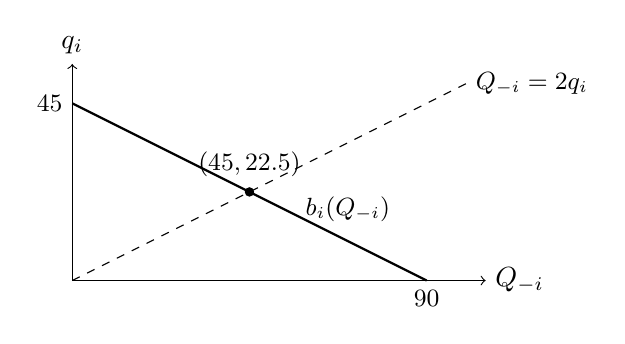
\begin{tikzpicture}[scale=0.05]
\draw[->] (0,0)--(105,0) node[right]{$Q_{-i}$};
\draw[->] (0,0)--(0,55) node[above]{$q_i$};
\draw[thick] (0,45)--(90,0);
\node[left] at (0,45){\small 45};
\node[below] at (90,0){\small 90};
\node at (70,18){\small $b_i(Q_{-i})$};
\draw[dashed] (0,0)--(100,50) node[right]{\small $Q_{-i}=2q_i$};
\fill (45,22.5) circle (1.2);
\node[above] at (45,24){\small $(45,22.5)$};
\end{tikzpicture}
\end{center}
The symmetric equilibrium is where the best response crosses the symmetry line $Q_{-i}=2q_i$.
\end{solution}
\item[4.3] Find the Cournot Nash equilibrium quantity of each firm $q^c$, total output $Q^c$ and price $p^c$.
\begin{solution}
Impose symmetry \emph{after} the FOC: $q^c=(90-2q^c)/2\Rightarrow 4q^c=90\Rightarrow q^c=22.5$. Then $Q^c=67.5$ and $p^c=100-67.5=32.5$.
\end{solution}
\item[4.4] Find each firm's profit, CS, PS, and TS.
\begin{solution}
$\pi_i=(32.5-10)(22.5)=506.25$. $PS=3\pi_i=1518.75$. $CS=\tfrac12(67.5)(100-32.5)=2278.125$. $TS=3796.875$.
\end{solution}
\item[4.5] Find the efficient outcome. Define and compute the Dead Weight Loss. Draw the market on the $p$--$Q$ plane showing CS, PS and DWL.
\begin{solution}
Efficient: $p=MC=10\Rightarrow Q^*=90$, $TS^*=\tfrac12(90)(90)=4050$.

\emph{Deadweight loss} is the total surplus lost relative to the efficient outcome, from trades worth more to buyers than they cost to produce that do not happen: $DWL=TS^*-TS^c=\tfrac12(90-67.5)(32.5-10)=253.125$.
\begin{center}
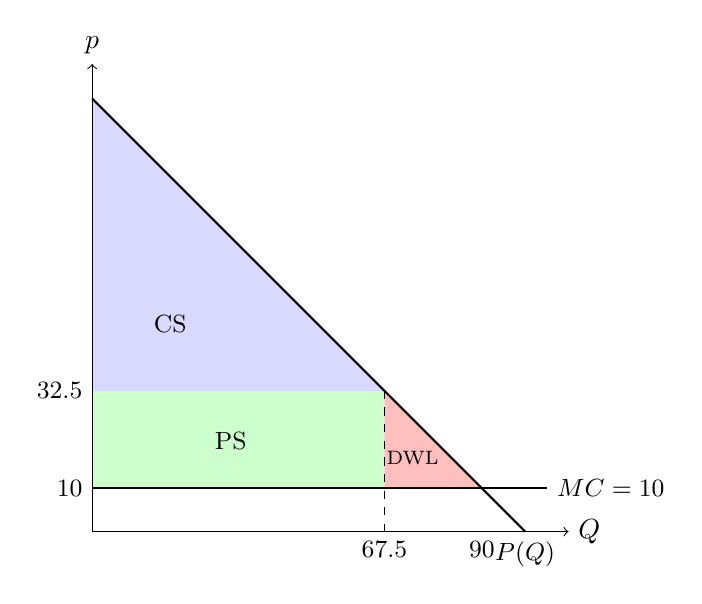
\begin{tikzpicture}[scale=0.055]
\fill[blue!15] (0,100)--(0,32.5)--(67.5,32.5)--cycle;
\fill[green!20] (0,10) rectangle (67.5,32.5);
\fill[red!25] (67.5,32.5)--(67.5,10)--(90,10)--cycle;
\draw[->] (0,0)--(110,0) node[right]{$Q$};
\draw[->] (0,0)--(0,108) node[above]{$p$};
\draw[thick] (0,100)--(100,0) node[below]{\small $P(Q)$};
\draw[thick] (0,10)--(105,10) node[right]{\small $MC=10$};
\draw[dashed] (67.5,32.5)--(67.5,0);
\node[left] at (0,32.5){\small 32.5};
\node[left] at (0,10){\small 10};
\node[below] at (67.5,0){\small 67.5};
\node[below] at (90,0){\small 90};
\node at (18,48){\small CS};
\node at (32,21){\small PS};
\node at (74,17){\scriptsize DWL};
\end{tikzpicture}
\end{center}
\end{solution}
\item[4.6] Suppose the three firms form a cartel that maximizes joint profit and splits output equally. Find the cartel output and each firm's profit. Is this a Nash equilibrium? Explain.
\begin{solution}
Joint profit $(100-Q)Q-10Q$ is maximized at $90-2Q=0$, so $Q^m=45$, $p^m=55$, and total profit is $45^2=2025$. Each firm produces $15$ and earns $675>506.25$.

This is \textbf{not} a NE. Holding the other two at $15$ each ($Q_{-i}=30$), firm $i$'s best response is $b_i(30)=(90-30)/2=30\ne15$. Deviating gives $Q=60$, $p=40$, and $\pi_i=30\cdot30=900>675$. Each firm ignores that its extra output lowers its rivals' profit, exactly as in the Prisoner's Dilemma. The cartel outcome is better for the firms but unstable. (It is also worse for society: its DWL is bigger.)
\end{solution}
\item[4.7] Generalize to $n$ firms with the same demand and costs. Find $q^c(n)$, $p^c(n)$ and $DWL(n)$. What happens as $n$ grows? What does this say about the effect of competition on efficiency?
\begin{solution}
With $Q_{-i}=(n-1)q$: $q=(90-(n-1)q)/2\Rightarrow q^c(n)=\dfrac{90}{n+1}$, $Q^c(n)=\dfrac{90n}{n+1}$, $p^c(n)=\dfrac{100+10n}{n+1}$.
\[DWL(n)=\tfrac12\Big(90-\tfrac{90n}{n+1}\Big)\Big(p^c(n)-10\Big)=\frac{90^2}{2(n+1)^2}=\frac{4050}{(n+1)^2}.\]
Check: $n=1$ (monopoly) gives $Q=45$, $p=55$; $n=3$ gives $DWL=253.125$. As $n\to\infty$, $p^c\to10=MC$, $Q^c\to90$ and $DWL\to0$. More firms means each firm's output decision has a smaller effect on price, so the underproduction distortion shrinks toward the competitive, efficient outcome.
\end{solution}
\end{description}
\end{document}
